\subsection{Управление яркостью светодиодной подсветки ЖКИ}

\begin{par}
Одним из основных параметров светодиодов является: яркость — величина,
равная отношению силы света к площади светящейся
поверхности, измеряемая в канделах на квадратный метр. \\

Спектральная характеристика светодиода выражает зависимость интенсивности
излучения от длины волны излучаемого света и дает представление о цвете
свечения светодиода. \\

Длина волны излучаемого света определяется разностью
энергий двух энергетических уровней, между которыми происходит переход
электронов на излучательном этапе процесса рекомбинации и определяется
исходным полупроводниковым материалом и легирующими примесями.
\end{par}

\subsubsection{Уменьшение яркости светодиода методом ШИМ}

\begin{par}
Наиболее простой способ уменьшения яркости светодиода - изменение прямого
тока или напряжения [http://www.e-neon.ru/user_img/pages/Dimming_InGaN_rus.pdf].
Но необходимо учитывать, что изменение этих параметров будет влиять на
длину волны излучаемого света, причём чем больше длинна волны, тем сильнее
выражен этот эффект.
Помимо тока, на длину волны оказывает влияние так же и температура.
Но это влияние не столь существенно и может игнорироваться.
\end{par}

\begin{par}
В схемах с использованием ШИМ через светодиод проходит последовательность импульсов.
Если частота следования импульсов более 200Гц, человеческий
глаз, обладающий инерционностью[TODO], будет ощущать непрерывное свечение
светодиода. Изменняя длительность и скважность импульса можно добиться того,
что зрение будет интегрировать и интерпретировать отдельные световые импульсы
как изменение силы света.
\end{par}

\begin{figure}[h]
	\center{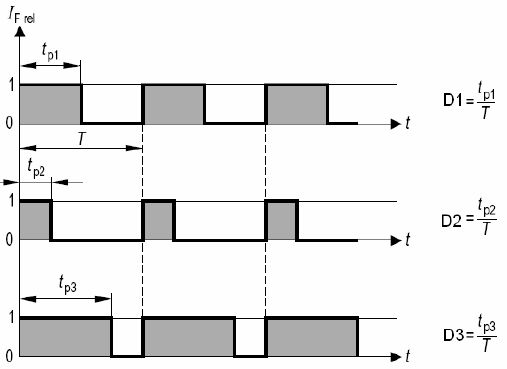
\includegraphics[bb=0 0 507 396]{led_pwm.png}}
	\caption{Управление яркосьтю светодиода ШИМ}
	\label{img:led_pwm}
\end{figure}

\begin{par}
При неизменном токе яркость свечения зависит от скважности
следующим образом: \\
    $$ D_2 < D_1 < D_3 $$

При этом, визуальная сила света будет меняться линейно при соответствующем
линейгном изменении скважности [TODO: откуда я взял эту информацию].
\end{par}

[TODO: А так же какова будет зависимость в чиселках]

